% !TeX root = ../main.tex

\chapter{论文相关基础知识}

%\section{引言}

本章将介绍深度学习隐私保护研究的基础知识。具体来说,本章将首先介绍深度学习在自然语言处理任务中的应用,包括任务的定义、常见的模型结构等内容。然后,介绍多方安全计算和差分隐私这两种在深度学习隐私保护中广泛使用的隐私保护技术,包括其定义、性质和常见的实现方式。最后,本文将介绍可信硬件Intel SGX,它可以为深度学习隐私保护提供一个安全可靠的执行环境。通过本章的介绍,读者可以全面了解本文所涉及的技术基础,并为后续章节的研究工作做好准备。

\section{基于深度学习的自然语言处理}

本节将介绍自然语言处理的形式化定义及任务描述与常见的深度学习模型结构。

%\subsection{自然语言处理的形式化定义} \label{NLP_Def}
%
%自然语言处理是一门语言学、计算机科学与人工智能领域的交叉学科,旨在让计算机理解、分析、生成和处理自然语言文本数据。在NLP中,文本被视为离散符号序列,记为$S=(w_1, w_2, ..., w_n)$,其中$w_i$表示文本中的第$i$个单词或标点符号。
%
%在NLP中,语言模型是一种基本的概率模型,用于预测给定文本序列的下一个单词或字符。语言模型可以表示为$p(w_i|w_1, w_2, ..., w_{i-1})$,即在已知前$i-1$个单词的情况下,预测第$i$个单词的概率。其中,$p(w_i|w_1, w_2, ..., w_{i-1})$可以通过训练数据集中的单词出现频率来计算。在具体实现时,通常采用神经网络模型来实现语言模型,如循环神经网络、长短时记忆网络(Long Short-Term Memory Network,LSTM)和Transformer等。
%
%除了语言模型,NLP中还有许多其他的模型和算法,这些模型和算法能够帮助处理自然语言文本数据,从而实现各种NLP任务。
%
%\subsection{自然语言处理任务介绍}
%
%自然语言处理是人工智能领域的一个重要分支,它致力于让计算机理解、解释和生成人类语言。基于深度学习的自然语言处理技术在过去几年取得了显著的进展,推动了一系列NLP任务的发展。以下是一些主要的NLP任务介绍。
%
%\begin{itemize}
%	\item [1)]
%	词法分析。词法分析是NLP的基本任务之一,主要包括分词、词性标注和命名实体识别。分词是将句子划分成有意义的词汇单元的过程。词性标注是为每个词汇单元分配一个词性标签,如名词、动词、形容词等。命名实体识别(NER)是识别文本中具有特定意义的实体,如人名、地名、机构名等。
%	\item [2)]
%	信息抽取。信息抽取旨在从非结构化文本中抽取结构化信息,主要任务包括关系抽取、事件抽取和实体链接。关系抽取是识别文本中命名实体之间的语义关系。事件抽取是识别文本中描述的事件及其相关实体。实体链接是将文本中的命名实体与知识库中的实体进行链接。
%	\item [3)]
%	机器翻译。机器翻译是将一种自然语言文本自动翻译成另一种自然语言文本的任务。机器翻译可以分为统计机器翻译(Statistical Machine Translation,SMT)、神经机器翻译(Neural Machine Translation,NMT)和基于预训练模型的翻译方法。SMT依赖于大量双语语料库,利用统计方法进行翻译建模。NMT使用神经网络,特别是编码器-解码器结构进行端到端的翻译建模。预训练模型如BERT\cite{BERT}和GPT\cite{GPT2, GPT3}等通过在大量单语和双语语料库上预训练,进一步提升了翻译性能。
%	\item [4)]
%	文本摘要。文本摘要任务是生成一个简洁、连贯且包含原始文本主要信息的摘要。文本摘要可以分为抽取式摘要和生成式摘要。抽取式摘要是从原文中选择关键句子或短语构成摘要,而生成式摘要是生成新的句子来表达原文的核心信息。深度学习技术在生成式摘要方面取得了显著进展,如使用编码器-解码器结构和预训练模型进行摘要生成。。
%	\item [5)]
%	语言生成。语言生成是自然语言处理的一个核心任务,它的目标是根据给定的输入生成符合语法、语义和篇章逻辑的自然语言文本。近年来,预训练语言模型(如GPT系列模型)在各种生成任务中取得了显著的成果,包括文本生成、对话生成、文本摘要等。预训练语言模型通过在大量文本数据上进行无监督训练,学习到了丰富的语言知识和生成能力。
%	\item [6)]
%	知识图谱。知识图谱是一种结构化的知识表示方法,它以图的形式表示实体及其之间的关系。知识图谱在自然语言处理中的应用包括实体链接、关系抽取、知识图谱补全等。深度学习技术在知识图谱领域的应用主要包括基于图神经网络的表示学习方法,以及将知识图谱与预训练语言模型相结合的方法。
%\end{itemize}

\subsection{自然语言处理的形式化定义及任务描述} \label{NLP_Def}

自然语言处理是一门语言学、计算机科学与人工智能领域的交叉学科,旨在让计算机理解、分析、生成和处理自然语言文本数据。在NLP中,文本被视为离散符号序列,记为$S=(w_1, w_2, ..., w_n)$,其中$w_i$表示文本中的第$i$个单词或标点符号。为了形式化地描述自然语言处理任务的内容,可以将其定义为从输入序列$S$到输出序列$T$的映射问题,即$T=f(S)$,其中函数$f$根据具体任务的需求进行定义。

在自然语言处理任务中,有许多具体的子任务,如词性标注、命名实体识别、句法分析、语义分析、文本分类、文本摘要、机器翻译、情感分析等。下面将通过一些具体的任务示例来详细描述这些任务的形式化定义:

\begin{itemize}
	\item [1)]
	词性标注(Part-of-Speech Tagging, POS Tagging):给定一个文本序列$S=(w_1, w_2, ..., w_n)$,词性标注任务的目标是为每个单词$w_i$分配一个词性标签$t_i$。输出序列$T=(t_1, t_2, ..., t_n)$,其中$t_i$表示第$i$个单词的词性标签。因此,词性标注任务可以定义为:$T = f_{\text{POS}}(S)$。
	\item [2)]
	命名实体识别(Named Entity Recognition, NER):给定一个文本序列$S=(w_1, w_2, ..., w_n)$,命名实体识别任务的目标是识别出序列中的命名实体(如人名、地名、组织名等)及其类型。输出序列$T=(e_1, e_2, ..., e_m)$,其中$e_i$表示一个命名实体及其类型。因此,命名实体识别任务可以定义为:$T = f_{\text{NER}}(S)$。
	\item [3)]
	文本分类(Text Classification):给定一个文本序列$S=(w_1, w_2, ..., w_n)$,文本分类任务的目标是为文本分配一个或多个类别标签。输出$T = (c_1, c_2, ..., c_k)$,其中$c_i$表示一个类别标签。因此,文本分类任务可以定义为:$T = f_{\text{TC}}(S)$。
	\item [4)]
	文本摘要(Text Summarization):给定一个文本序列$S=(w_1, w_2, ..., w_n)$,文本摘要任务的目标是生成一个较短的文本序列,包含原始文本的主要信息。输出序列$T=(w'_1, w'_2, ..., w'_m)$,其中$w'i$表示摘要中的第$i$个单词或标点符号,且$m \leq n$。因此,文本摘要任务可以定义为:$T = f_{\text{TS}}(S)$。
	\item [5)]
	机器翻译(Machine Translation, MT):给定一个源语言文本序列$S=(w_1, w_2, ..., w_n)$,机器翻译任务的目标是将其翻译成目标语言文本序列。输出序列$T=(w'_1, w'_2, ..., w'_m)$,其中$w'_i$表示目标语言文本中的第$i$个单词或标点符号。因此,机器翻译任务可以定义为:$T = f_{\text{MT}}(S)$。
	\item [6)]
	情感分析(Sentiment Analysis):给定一个文本序列$S=(w_1, w_2, ..., w_n)$,情感分析任务的目标是判断文本中表达的情感极性(如正面、负面或中性)。输出$T = (p)$,其中$p$表示情感极性标签。因此,情感分析任务可以定义为:$T = f_{\text{SA}}(S)$。
\end{itemize}

通过以上描述,可以看到自然语言处理任务涉及多种子任务,每个子任务都可以用一个特定的函数$f$来形式化地描述其输入和输出。在实际应用中,根据任务的具体需求,使用者可以选择合适的模型和方法来实现这些函数。


\subsection{常见的自然语言处理模型结构}

深度学习技术在自然语言处理领域取得了显著的进展,特别是在文本表示和序列建模方面。以下是一些常见的深度学习模型结构,它们在自然语言处理任务中具有广泛的应用。

\begin{itemize}
	\item [1)]
	循环神经网络(Recurrent Neural Networks, RNN):RNN是一种适用于处理序列数据的神经网络结构。它具有内部状态,可以在处理长序列时保留之前时间步的信息。RNN在词性标注、命名实体识别、机器翻译等任务中有广泛应用。
	\item [2)]
	长短时记忆网络(Long Short-Term Memory, LSTM):LSTM是一种特殊的RNN结构,它通过引入门控机制来解决RNN在处理长序列时的梯度消失和梯度爆炸问题。LSTM在许多自然语言处理任务中取得了很好的效果,如语言模型、文本摘要、机器翻译等。
	\item [3)]
	门控循环单元(Gated Recurrent Units, GRU):GRU是另一种特殊的RNN结构,它与LSTM类似,但具有更简单的门控结构。GRU在某些自然语言处理任务中表现出与LSTM相近的性能,但计算复杂度较低。
	\item [4)]
	卷积神经网络(Convolutional Neural Networks, CNN):CNN是一种广泛应用于计算机视觉领域的神经网络结构。然而,近年来研究发现,CNN也可以应用于自然语言处理任务,如文本分类、情感分析等。通过使用一维卷积操作,CNN可以捕捉文本中的局部特征。
	\item [5)]
	Transformer:Transformer是一种基于自注意力(Self-Attention)机制的神经网络结构。它摒弃了RNN和CNN中的循环和卷积操作,通过自注意力机制捕捉序列中的长距离依赖关系。Transformer在诸如机器翻译、语义角色标注和依存句法分析等自然语言处理任务中取得了显著的成果。
	
\end{itemize}



%在深度学习模型中,常见的用于NLP任务的模型结构包括循环神经网络、长短期记忆网络、门控循环单元网络(Gated Recurrent Unit Network,GRU)和Transformer。RNN和LSTM是最早被应用于NLP任务的深度学习模型,它们的优势在于可以处理变长序列数据。GRU是对LSTM的改进,能够在保持同样效果的情况下减少计算量。而Transformer网络则采用了注意力机制,能够更好地处理长距离依赖关系,因此在机器翻译任务中表现非常出色。
%
%这些模型的共同特点是它们都是端到端(end-to-end)的模型,其输入数据是一段文本序列,输出则是一个对应的文本序列。在NLP任务中,这些模型通常被用于生成文本,例如文本摘要、对话系统和机器翻译等任务。在本文中,我们将研究如何在保护训练数据和生成的文本隐私的同时,使用这些深度学习模型来生成医学文本。

\section{多方安全计算}


\subsection{多方安全计算定义}

多方安全计算技术的研究主要是针对无可信第三方的情况下,多个参与者如何在不暴露己方数据的情况下安全地计算一个约定函数的问题。多方安全计算协议分为信息论安全和密码学安全。如果协议对于拥有无限计算能力的攻击者来说是安全的,那么它被称为信息论安全或无条件安全。如果协议只对拥有多项式计算能力的攻击者是安全的,则称为密码学安全或条件安全。多方安全计算协议的目的是实现一些特定的计算任务。多方安全计算的目的是实现一些特定的计算任务,例如比较、加密、解密、排序、计数、求和等。在多方安全计算中,每个参与方持有自己的输入数据,并且希望在不泄露私有数据的情况下与其他方共同计算结果。

多方安全计算具有以下性质:

\begin{itemize}
	\item [1)]
	正确性。采用多方安全计算协议计算的结果与直接使用明文数据计算的结果相同。具体而言,针对输入为$x$,运算法则为$Q$的一个多方安全计算协议$M$,有
	$$P[M(x,f)=Q(x)]=1\text{。}$$
	
	假设有 $n$ 个参与者,分别为 $P_1, P_2, ..., P_n$,他们各自持有输入 $x_1, x_2, ..., x_n$,并希望在不泄露私密输入的情况下计算某个函数 $f(x_1, x_2, ..., x_n)$。多方安全计算协议(MPC)是指在参与者之间进行的一系列通信和计算过程,使得每个参与者最终可以获得函数 $f$ 的输出,同时不会泄露任何其他参与者的输入。
	\item [2)]
	隐私性。任何多方安全计算协议参与方不能获得除协议规定内的额外信息。具体而言,所有参与方$P=(p_1, p_2, \dots, p_n)$,对于参与者$p_k\in P$,使用参与者数据$F=(f_1, f_2, \dots, f_n)$输出结果为$L$的多方安全计算协议$M$,存在一个可忽略的函数$\epsilon$,有下式成立:
	$$P_{p_k}(f_{i,i\neq k}|L=M(F))+P_k(f_k)\leq P(f_{i,i\neq k})+\epsilon\text{。}$$
	
\end{itemize}


\subsection{多方安全计算的安全性}
在介绍了多方安全计算的定义后,为理解其安全性,下面介绍多方安全计算场景中不同的安全假设。

\begin{itemize}
	\item [1)]
	半诚实(Semi-honest)参与者假设:在这种假设下,半诚实的参与者会遵守协议并诚实地执行计算,但他会记录协议执行的上下文来获得更多关于隐私数据的信息。尽管这种安全假设对于参与者的行为作出了相对严格的假设,但在实际场景中仍然相对较强。
	\item [2)]
	恶意(Malicious)参与者假设:在这种安全假设下,协议不对恶意参与者的行为作任何假设。恶意参与者可以采取偏离、中断或中止协议等手段,从而获取其他参与者的隐私输入信息,因此这种安全假设比半诚实假设更为严格。
\end{itemize}

现实-理想框架是一种多方安全计算安全性的形式化框架,其使用了一个包含所有安全需求的“理想世界”,通过现实世界与理想世界之间的对应关系定义多方案去计算。

理想世界中,参与方$P(p_1, p_2, \dots, p_n)$将各自的输入$F=(f_1, f_2, \dots, f_n)$发送给一个可信第三方$S$,$S$执行函数$Q$,并将计算结果$Q(F)$返回给所有参与方。假设存在一个在理想世界中的攻击者$A$,其可以控制除参与方其$p_k$外任意数量的参与方$P_A\subset P$其中$p_k\notin P_A$,它试图通过各种攻击手段获取$p_k$的输入。由于攻击者$A$无法控制可信第三方$S$,因此攻击者$A$无法获得除$Q(F)$外的任何信息。

由于现实世界中不存在上述可信第三方$S$,各参与方需要相互交互以完成计算。在参与方$p_i$以其隐私输入$f_i$、当前状态的中间值$h_i$、接收到的所有信息$Context$、随机数$R_i$、安全性参数$\kappa$作为输入时,通过执行函数$\pi_i$,获得新的中间值或者输出。

如果攻击者在现实世界达到的攻击效果与其在理想世界的攻击效果相同,那么可以将该协议认为是在现实世界中安全的,即协议使得其在现实世界中提供的安全性与在理想世界中提供的安全性等价。

\begin{definition}{}
	记$\pi$为一个协议,$Q$为一个函数,$P_A$为被攻击者$A$控制的参与方集合,$\text{Sim}$为仿真算法,定义如下两种协议。
	\begin{itemize}
		\item [$\cdot$]
			$\text{Real}_\pi(\kappa,P_A;f_1,f_2,\cdots,f_n)$:在安全性参数$\kappa$下参与方$P=(p_1, p_2, \dots, p_n)$使用各自隐私数据入$F=(f_1, f_2, \dots, f_n)$在真实世界执行的协议。记$V={v_1, v_2, \dots, v_n}$为参与方$P$的最终视图,即$\{v_i|i\in (1,2,\cdots,n)\}$;$y={y_1, y_2, \dots, y_n}$为参与方$P$的输出结果。
		\item [$\cdot$]
			$\text{Ideal}_{Q,\text{Sim}}(\kappa,P_A;f_1,f_2,\cdots,f_n)$:模拟世界中在安全性参数$\kappa$下参与方$P(p_1, p_2, \dots, p_n)$使用各自隐私数据入$F=(f_1, f_2, \dots, f_n)$在仿真算法$\text{Sim}$与函数$Q$的计算下执行的协议,其输出为$\text{Sim}(P_A,\{(f_i,y_i)\in P_A\})$			
	\end{itemize}

\end{definition}

在参与方是半诚实的假设下,其会诚实地执行协议,但可能会从接收到的信息中尝试推断更多的信息。

\begin{definition}{}
	给定协议$\pi$,$Q$为一个函数,$P_A$为被攻击者$A$控制的参与方集合,如果存在一个为仿真算法$\text{Sim}$,对于攻击者$A$控制的所有参与方集合$P_A$以及所有的输入$F=(f_1, f_2, \dots, f_n)$,概率分布$Real_\pi(\kappa,P_A;f_1,f_2,\cdots,f_n)$与$\text{Ideal}_{Q,\text{Sim}}(\kappa,P_A;f_1,f_2,\cdots,f_n)$在$\kappa$下不可区分,则称此协议在半诚实攻击者的攻击下安全地实现了函数$Q$。
\end{definition}

在参与方是恶意的假设下,其不仅会从接收到的信息中尝试推断更多的信息,而且还可以任意破坏、偏离协议。这里使用A表示攻击程序,用Corr($A$)表示被现实世界中的攻击者攻陷的参与方集合,用Corr(Sim)表示被理想世界中的攻击者Sim攻陷的参与方集合。与上述半诚实安全性的方式类似,定义现实世界与理想世界下的概率分布:
\begin{itemize}
	\item [$\cdot$]
	$\text{Real}_{\pi,A}(\kappa;\{x_i|i\notin \text{Corr}(A)\})$:在安全性参数$\kappa$下,未被攻陷的参与方城市地使用给定的隐私输入执行协议,而被攻陷的参与方Corr(A)的信息可以由A进行篡改,并参与到后续的协议执行过程中。记$v_i$为参与方的最终视图,即$\{v_i|i\in \text{Corr}(A)\}$;$y_i$为诚实参与方$p_i$的输出结果,即$\{y_i|i\notin \text{Corr}(A)\}$。
	\item [$\cdot$]
	$\text{Ideal}_{Q,\text{Sim}}(\kappa;\{x_i|i\notin \text{Corr}(A)\})$:模拟世界中,在安全性参数$\kappa$下,在包含攻陷方输入$\{x_i|i\in \text{Corr}(A)\}$的数据上执行$\text{Sim}$协议。计算$(y_1,\cdots,y_n)\leftarrow Q(f_1,\cdots,f_n)$后,将$\{y_i|i\notin \text{Corr}(A)\}$发送给$\text{Sim}$。记$V^*$为$\text{Sim}$最终输出,即各参与方的仿真视图集合。
\end{itemize}

\begin{definition}{}
	给定协议$\pi$与函数$Q$,对任意一个现实世界中的攻击者$A$,存在一个满足$\text{Corr}(A)\Longleftrightarrow \text{Corr}(\text{Sim})$的仿真者$\text{Sim}$,使得对于诚实参与方的所有输入$\{x_i|i\notin \text{Corr}(A)\}$,概率分布$\text{Real}_{\pi,A}(\kappa;\{x_i|i\notin \text{Corr}(A)\})$与$\text{Ideal}_{Q,\text{Sim}}(\kappa;\{x_i|i\notin \text{Corr}(A)\})$在$\kappa$下不可区分,则称此协议在恶意攻击者的攻击下安全地实现了函数$Q$。
\end{definition}

\section{差分隐私}

差分隐私\cite{DP}是一种保护隐私的方法,其基本思想是在不泄露个体信息的前提下,通过添加一定的噪声,使得查询结果的公开不会泄露个体的隐私信息。

\subsection{差分隐私定义与性质}

%差分隐私是一种保护个人隐私的技术,在不泄露个人隐私的前提下对数据进行分析和处理。具体来说,如图\ref{DP_demo}所示,其限制单条数据对算法输出的影响,即无论算法使用的数据集中包含某个特定个体与否,输出的结果都是相似的。这样保证了即使公开了算法在某特定数据集上的结果,也对数据集中的数据有着定量的隐私保护。下面给出差分隐私的具体定义。

差分隐私是一种保护个人隐私的技术,它可以在不泄露个人隐私的前提下对数据进行分析和处理。具体来说,如图 \ref{DP_demo} 所示,差分隐私通过限制单条数据对算法输出的影响来保护个人隐私,即无论数据集中是否包含特定个体,算法的输出结果不可区分。这种保护方式确保了即使公开了算法在某个特定数据集上的结果,数据集中的数据仍然受到定量的隐私保护。差分隐私的具体定义如下。

\begin{figure}[h]
	\centering
	%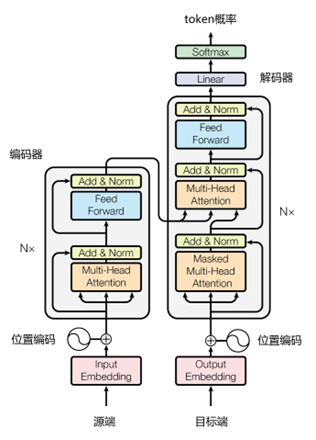
\includegraphics[width=1\textwidth]{figures/Transformer_Structure.png}
	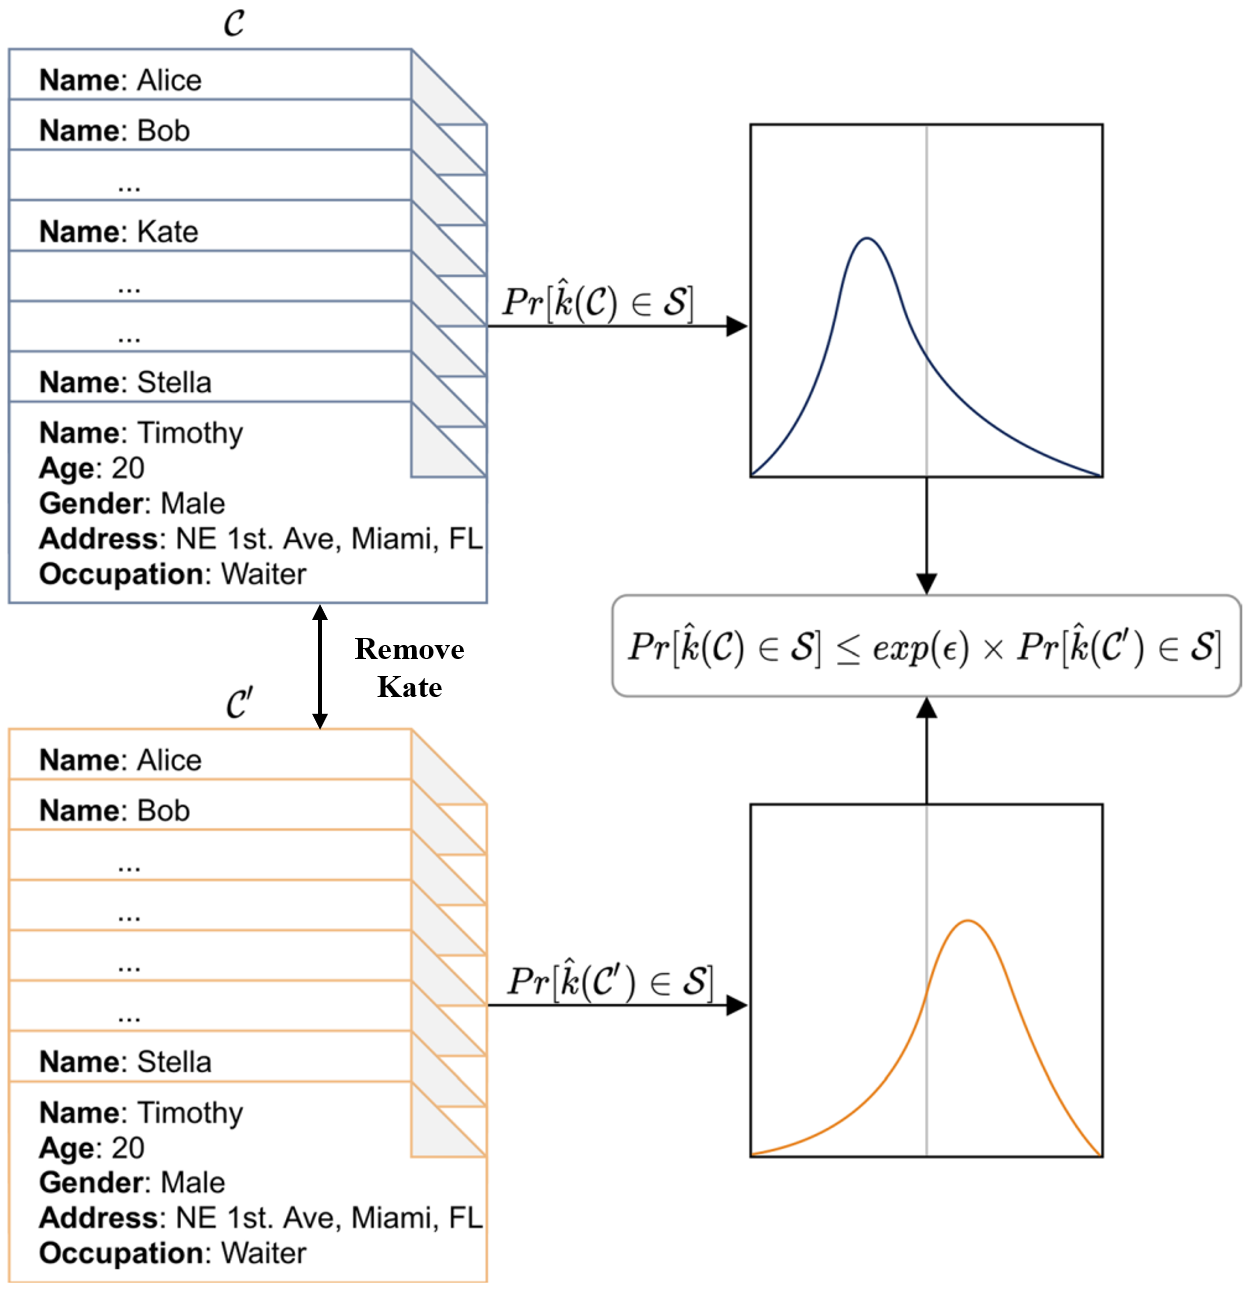
\includegraphics[width=0.8\linewidth]{figures/DP.png}
	\caption{差分隐私算法示意图}
	\label{DP_demo}
\end{figure}

\begin{definition}
	(近邻数据集\cite{dwork2006our})若数据集$D$与$D'$仅有一条记录不同,则称$D$与$D'$为近邻数据集。
\end{definition}



\begin{definition}
	($\epsilon$-差分隐私\cite{dwork2006our})对于任意近邻数据集$D$与$D'$以及任意的输出结果$S$,若随机算法$M$满足
	\begin{equation}
		\label{eps-dp}
		\mathop{Pr}[\mathcal{M}(D) = S] \leq e^{\epsilon} \cdot \mathop{Pr}[\mathcal{M}(D') = S]\text{,}
	\end{equation}
	则称$M$满足$\epsilon$-差分隐私。其中$\epsilon$表示隐私预算,它是衡量隐私保护程度的指标,$\epsilon$越小表示算法的隐私保护程度越高,反之$\epsilon$越大,算法在近邻数据集的结果之间的差别也越大,隐私保护程度便越低。
\end{definition}

式 \ref{eps-dp} 的条件在实际场景中往往过于苛刻,导致算法的可用性很差。因此,可以适当放宽$\epsilon$-差分隐私的要求,即松弛一下它的边界,这样就有了$(\epsilon, \delta)$-差分隐私。

\begin{definition}
	($(\epsilon, \delta)$-差分隐私\cite{Algorithmic_Foundations_of_DP})对于任意近邻数据集$D$与$D'$以及任意的输出结果$S$,若随机算法$M$满足
	\begin{equation}
		\label{eps-delta-dp}
		\mathop{Pr}[\mathcal{M}(D) = S] \leq e^{\epsilon} \cdot \mathop{Pr}[\mathcal{M}(D') = S] + \delta\text{,}
	\end{equation}
	则称$M$满足$(\epsilon, \delta)$-差分隐私。其中$\epsilon$同样表示隐私预算,而$\delta$为一个概率,算法在$1-\delta$的概率下满足式(\ref{eps-dp}),即只有至多$\delta$的概率不满足式(\ref{eps-dp}),这便要求$\delta$值很小,在数据集样本为$n$的情况下\cite{Mechanism_DP},需要$\delta<\frac{1}{n}$。$\epsilon$-差分隐私可以被视为$\delta=0$的$(\epsilon, \delta)$-差分隐私。
\end{definition}

%差分隐私满足以下几个性质\cite{Algorithmic_Foundations_of_DP}:
%\begin{itemize}
%	\item[$\bullet$]不可区分性:对于任意两个数据集$D$和$D'$,它们的任意一行的数据只相差一个,输出结果的分布也只相差一个,使得攻击者无法确定输出结果与哪个数据集相关。
%	\item[$\bullet$]增量脱敏性:任意对数据集进行的小的修改,对于隐私的影响也不会太大。
%	\item[$\bullet$]组合性:对于多次使用同样的差分隐私算法,每次使用的隐私预算$\epsilon$可以累加。
%	\item[$\bullet$]先验知识不增加隐私风险:差分隐私不受先验知识的影响,攻击者掌握了更多的先验知识,也不会增加隐私风险。
%\end{itemize}

下面给出一些形式化定义的定理。

\begin{theorem}\cite{Algorithmic_Foundations_of_DP}
	若随机算法$M_1$满足$(\epsilon, \delta)$-差分隐私,则对于任意算法$M_2$,有$M_2(M_1(\cdot))$满足$(\epsilon, \delta)$-差分隐私。
\end{theorem}

\begin{proof}
	对于$\forall S\in Range(M_2)$,记$Y=\{y|M_2(y)=S\}$,则
	\begin{align}
	\mathop{Pr}[M_2(M_1(D))=S]&=\mathop{Pr}[M_1(D)\in Y]\notag\\
	&\leq e^\epsilon \mathop{Pr}[M_1(D')\in Y]+\delta\notag\\
	&=\mathop{Pr}[M_2(M_1(D'))=S]+\delta\notag
	\end{align}\text{。}
\end{proof}

\begin{theorem}\cite{Algorithmic_Foundations_of_DP}
	若随机算法$M_i$满足$(\epsilon_i, \delta_i)$-差分隐私,其中$i=\{1,2,\cdots,n\}$,则算法$M(D)=(M_1(D),M_2(D,\cdots,M_n(D))$满足$(\sum_{i=1}^{n}\epsilon_i, \sum_{i=1}^{n}\delta_i)$-差分隐私。
\end{theorem}

%本文不加证明地给出以下定理。
%
%\begin{theorem}\cite{Algorithmic_Foundations_of_DP}
%	若随机算法$M_i$满足$(\epsilon, \delta)$-差分隐私,其中$i=\{1,2,\cdots,n\}$,则算法$M(D)=(M_1(D),M_2(D,\cdots,M_n(D))$满足$(\epsilon', n\delta+\delta')$-差分隐私。其中
%		$$\epsilon'=\sqrt{2n\ln(\frac{1}{\delta'})+n\epsilon(e^\epsilon-1)}$$\text{。}
%\end{theorem}


\subsection{常见的差分隐私实现}

差分隐私的实现方法有很多,包括基于噪声的加噪算法、基于随机投影的扰动算法、基于数据扰动的数据变形算法等。其中,添加噪声的加噪算法应用最为广泛,具体包括以下几种方法:拉普拉斯机制\cite{LaplaceM}、高斯机制\cite{Algorithmic_Foundations_of_DP}与指数机制\cite{Mechanism_DP}。下面首先介绍两种全局敏感度的概念,然后一次介绍上述机制的概念。

\begin{definition}
	(L1全局敏感度\cite{Algorithmic_Foundations_of_DP})对于近邻数据集$D$与$D'$,函数$f$的L1全局敏感度$\Delta_1f$的定义为:
	\begin{equation}
		\Delta_1f=max_{D,D'}||f(D)-f(D')||_1\text{。}
	\end{equation}
\end{definition}

\begin{definition}
	(L2全局敏感度\cite{Algorithmic_Foundations_of_DP})对于近邻数据集$D$与$D'$,函数$f$的L2全局敏感度$\Delta_2f$的定义为:
	\begin{equation}
		\Delta_2f=max_{D,D'}||f(D)-f(D')||_2\text{。}
	\end{equation}
\end{definition}


(1)拉普拉斯机制

拉普拉斯机制是一种添加噪声的差分隐私算法,它的基本思想是为每个查询结果添加一个服从拉普拉斯分布的噪声,从而保证查询结果的隐私性。

%具体地,对于查询结果 $q$,拉普拉斯机制会向其添加一个噪声值 $\Delta q$,其服从如下的拉普拉斯分布:
%
%$$ P(\Delta q = x) = \frac{\varepsilon}{2b} \exp\Big(-\frac{|x|}{b}\Big) $$
%
%其中,$\varepsilon$ 为差分隐私参数,$b$ 为拉普拉斯分布的尺度参数,控制噪声的大小。

\begin{definition}
	(拉普拉斯分布)均值为0,方差为$d$的拉普拉斯概率密度函数为:
	\begin{equation}
		\text{Laplace}(x, d)=\frac{1}{2d}\exp\left(-\frac{|x|}{d}\right)\text{。}
	\end{equation}
\end{definition}

\begin{theorem}
	(拉普拉斯机制\cite{dwork2006calibrating})对于任意函数$f$,其L1全局敏感度为$\Delta_1f$,算法$M=f(D)+\text{Laplace}(\frac{\Delta_1f}{\epsilon})$满足$\epsilon$-差分隐私。
\end{theorem}

(2)高斯机制

高斯机制是一种添加噪声的差分隐私算法,它的基本思想是为每个查询结果添加一个服从高斯分布的噪声,从而保证查询结果的隐私性。与拉普拉斯机制不同的是,高斯机制引入的噪声值是连续的,并且其分布更加平滑。

%\begin{definition}
%	(高斯分布)均值为$\mu$,方差为$\sigma$高斯分布的概率密度函数为:
%	\begin{equation}
%		f(x)=\frac{1}{\sqrt{2\pi\sigma}}\exp(-\frac{(x-\mu)^2}{2\sigma^2})\text{。}
%	\end{equation}
%\end{definition}

\begin{theorem}
	(高斯机制\cite{Algorithmic_Foundations_of_DP})对于任意函数$f$,其L2全局敏感度为$\Delta_2f$,加上高斯分布噪声的算法$M=f(D)+N(0,\Delta_2f\sigma^2)$满足$(\epsilon, \delta)$-差分隐私。其中$\epsilon<1$,且
	$$\delta\geq \frac{4}{5}\exp\left(-\frac{(\sigma\epsilon)^2}{2}\right)\text{。}$$
\end{theorem}

%具体地,对于查询结果 $q$,高斯机制会向其添加一个服从如下高斯分布的噪声值 $\Delta q$:
%
%$$ P(\Delta q = x) = \frac{1}{\sqrt{2\pi}\sigma}\exp\Big(-\frac{x^2}{2\sigma^2}\Big) $$
%
%其中,$\sigma$ 为高斯分布的标准差,控制噪声的大小。

(3)指数机制

指数机制是一种添加噪声的差分隐私算法,它的基本思想是将查询结果的隐私性与其“有用性”相平衡,从而选择最优的查询结果。具体地,指数机制会对每个查询结果赋予一个得分值,得分越高表示该结果越有用,然后根据指数分布的概率密度函数从所有结果中以概率 $p_i$ 选择结果 $i$,其中

$$ p_i = \frac{\exp(\epsilon s_i)}{\sum_{j=1}^{n}\exp(\epsilon s_j)} \text{。}$$

上式中$s_i$ 为结果 $i$ 的得分值,$\epsilon$ 为差分隐私参数,控制查询结果的隐私性和“有用性”之间的平衡。


\begin{theorem}
	(指数机制\cite{mcsherry2007mechanism})可用性函数$u$对算法$M$在数据集$D$上的任何输出数值$y$给出一个可用性评估值$u(D,y)\in R$,若算法$M$输出结果$y$的概率正比于$exp(\frac{\epsilon u(D,y)}{2\delta u})$,即
	\begin{equation}
		\mathop{Pr}[M(D)=y]=\frac{\exp(\frac{\epsilon u(D,y)}{2\delta u})}{\sum_{y'\in Y}\exp(\frac{\epsilon u(D,y')}{2\delta u})}\text{。}
	\end{equation}
其中$\Delta u = max_{\{\forall y, D, D'\}}|u(D,y)-u(D',y)|$,则算法$M$满足$\epsilon$-差分隐私。
\end{theorem}

\section{可信硬件Intel SGX}

%传统的计算机系统存在着一些安全漏洞,例如操作系统和应用程序都可以访问系统中的所有资源,从而可能泄露用户数据或应用程序的机密信息。为了解决这一问题,研究者们提出了一种新型的安全计算模式,称之为可信计算。可信计算是指对计算机系统中所有可信任和不可信任的组件进行验证和安全性保护,以保证在不可信的环境中进行安全计算。为了实现可信计算,产生了一种特殊的可信硬件,即安全芯片。安全芯片是一种专用的微处理器,其硬件架构和安全设计考虑了保护计算机系统中敏感数据和代码的安全问题。

可信执行环境是一种在计算机系统中创建的隔离环境,它提供了比普通操作系统更高的安全性和可信度。可信执行环境的目的是保护系统中的敏感数据和代码,以及提供隔离环境来执行受保护的计算,防止恶意软件和攻击者对系统进行攻击和窃取信息。在可信执行环境中,所有的敏感数据和代码都可以得到保护。TEE提供了一个独立的内存空间,其中的代码和数据与主机操作系统完全隔离,从而可以保护这些数据和代码不受到主机操作系统和其他应用程序的干扰。TEE还提供了安全的输入和输出通道,使得敏感数据能够安全地进入和离开可信执行环境。在可信执行环境中运行的应用程序必须经过验证和授权才能被允许运行,这样可以防止不受信任的应用程序进入可信执行环境。同时,可信执行环境还提供了追踪和审计功能,用于记录TEE中的所有活动,这可以提供重要的证据来追踪和调查安全事件。

%\subsection{SGX的保护机制}

Intel SGX是英特尔公司推出的一种可信计算技术,其目的是提供一种安全的硬件环境,以保护计算机系统中的敏感数据和代码。Intel SGX是一种硬件扩展,它通过在处理器中引入特定的安全硬件,创建一种安全的执行环境,可以在这个环境中运行代码和数据,以实现可信计算。Intel SGX在保护数据和代码时,采用了一种称为“隔离执行”的技术,该技术可以保证数据和代码在安全的执行环境中被隔离开来,从而防止非授权的访问和修改。同时,Intel SGX还提供了一种特殊的机制,称为飞地(Enclave),用于实现在执行环境中运行的应用程序的安全性保护。%如图 \ref{SGX_Program} 所示,执行程序被划分为可信与不可信部分,为保护数据隐私,不可信代码通过调用ecall来使Enclave执行可信代码\textcircled{3},可信代码执行完成后通过调用ocall来返回不可信部分\textcircled{5}。

%\begin{figure}[h]
%	\centering
%	%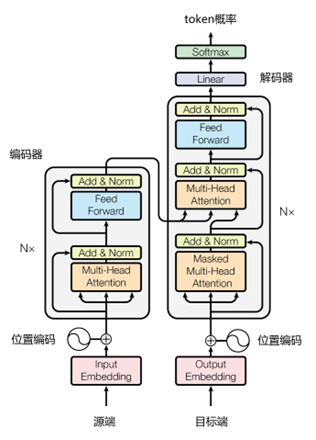
\includegraphics[width=1\textwidth]{figures/Transformer_Structure.png}sep_exeEncalveE
%	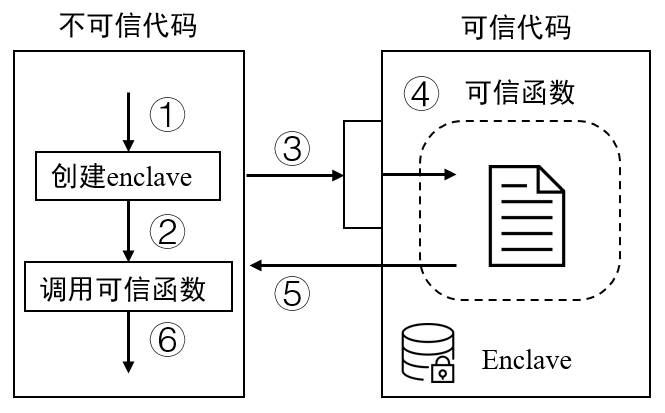
\includegraphics[width=0.6\linewidth]{figures/SGX_Program.png}
%	\caption{SGX应用程序划分与执行流程}
%	\label{SGX_Program}
%\end{figure}

(1)隔离执行

SGX安全体系结构保证Enclave与其他运行在Enclave之外的软件隔离执行,包括操作系统。通过隔离,可以保证Enclave控制流的完整性,并且被执行的Enclave 的内部机密数据不会被任何对手观察到。隔离是通过处理器执行的保护机制实现的。Enclave的代码和数据存储在称为 EPC(Enclave Page Cache)的硬件保护内存区域中,该内存驻留在处理机保留内存(Processor ReservedMemory, PRM)中,如图 \ref{Sep_Exe} 所示,其中内存加密引擎(Memory Encryption Engine, MEE)对Enclave中的数据进行加解密,在数据写入内存时加密,在读入Enclave时解密。PRM是动态随机存储器(Dynamic RandomAccess Memory)的一个子集,操作系统、应用程序或直接内存访问器都不能访问它。PRM保护是基于处理器中的一系列内存访问检查,非 Enclave软件仅允许访问PRM范围之外的内存区域,而Enclave代码可以访问非PRM内存和Enclave拥有的EPC页面。

\begin{figure}[h]
	\centering
	%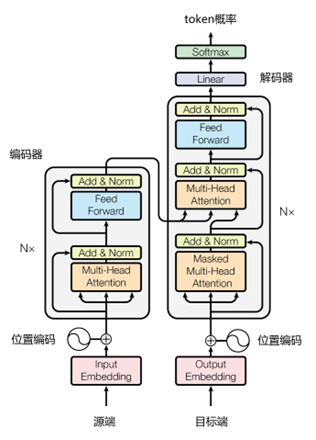
\includegraphics[width=1\textwidth]{figures/Transformer_Structure.png}sep_exeEncalveE
	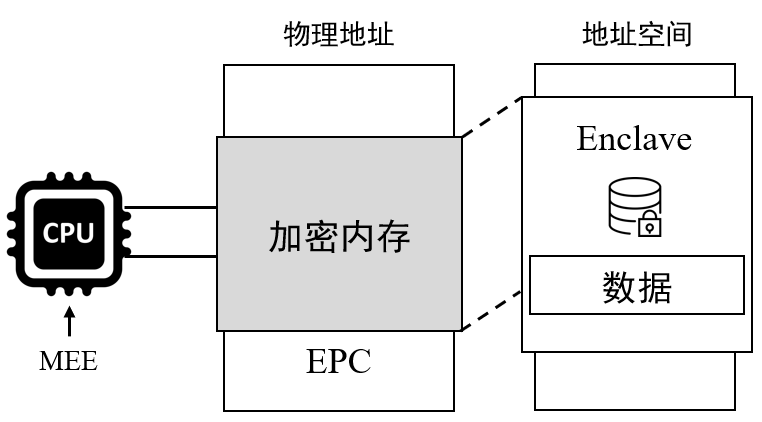
\includegraphics[width=0.6\linewidth]{figures/sep_exe.png}
	\caption{可信硬件SGX飞地的隔离执行示意图}
	\label{Sep_Exe}
\end{figure}

(2)远程认证

在构建Enclave时,Enclave的测度(MeasuRement of Enclave, MRE),即Enclave初始代码和数据的安全哈希值,由处理器生成,该哈希值保证Enclave的完整性。SGX提供了两种类型的身份认证方式:一种是平台内部 Enclave间的认证,称为本地认证(Local Attestation);另一种是平台间的认证,称为远程认证(Remote Attestation)。被认证的Enclave通过调用EREPORT指令生成报告(Report Structure),EREPORT是SGX提供的一个硬件指令,只有运行在SGX平台上的合法Enclave 才可以调用并生成报告,其中会包含该Enclave的测度,其完整性由基于Intel SGX硬件产生的密钥保护。

%远程认证过程需要引入一个特殊的 Enclave,称为QE(Quoting Enclave) ,QE是由Intel开发的特权级Enclave,只有QE 才可以访问认证密钥(AttestationKey)。被认证的Enclave 将报告发送给QE后,QE会验证报告是否由合法的Enclave产生。验证通过后,QE会使用认证密钥(Attestation Key)对报告进行签名,从而生成引用(Quote Structure),这里的签名方案基于EPID (EnhancedPrivacy IDentification),用于保护签名硬件的隐私。如果有一个远程认证方希望验证该Enclave,则该远程认证方将引用发送给Intel认证服务器(Intel AttestationService,IAS),IAS会验证该引用是否产生于合法的Intel SGX平台,并对引用签名生成IAS报告(IAS Report Structure),并将IAS报告发送给远程认证方。远程认证方通过IAS认证结果判断被认证的Enclave是否是合法的 Intel SGX平台上的,并且验证报告中的测度字段是否和与自己预期的测度值相等,从而完成一次远程认证。

每个SGX处理器都有一个根密封密钥(Root Seal Key, RSK),其在制造过程中嵌入,用于生成与Enclave 身份绑定的密封密钥(Seal Key)。SGX有一个称为密封的过程,是使用密封密钥加密和验证Enclave数据以便持久存储。Enclave可以使用EGETKEY指令从RSK派生出密封密钥,并且该密封密钥具有唯一性,即与同一平台的不同Enclave或不同平台的任何Enclave都不同。


%\subsection{针对SGX的攻击}

%\section{本章小结}
%
%本章首先从基于深度学习的NLP展开,介绍了NLP的定义与任务的分类。然后介绍了后续用于保护医学文本生成任务的隐私保护技术,包括了多方安全计算、差分隐私与可信硬件SGX。本章为后续的工作进行了铺垫,提供了前进方向。